\section{PROCEDIMENTOS METODOLÓGICOS}

Para alcançar o objetivo de classificar os comentários pejorativos em vídeos infantis do Youtube, os passos a seguir foram realizados ao longo da execução do trabalho.
Uma ilustração da ordem de execução dos passos é descrita na Figura \ref{fig:metodologia}.

\begin{itemize}
    \item Escolha dos vídeos;
    \item Coleta de dados;
    \item Pré-Processamento;
    \item Definição dos critérios de classificação;
    \item Treinamento do modelo de classificação;
    \item Avaliação do modelo de classificação;
    \item Criação de extensão para Google Chrome;
    
\end{itemize}

\begin{figure}[H] %use h para forçar que a figura fique abaixo do texto
	\caption{\label{fig:metodologia} Ilustração do procedimento metodológico}
	\begin{center}
	    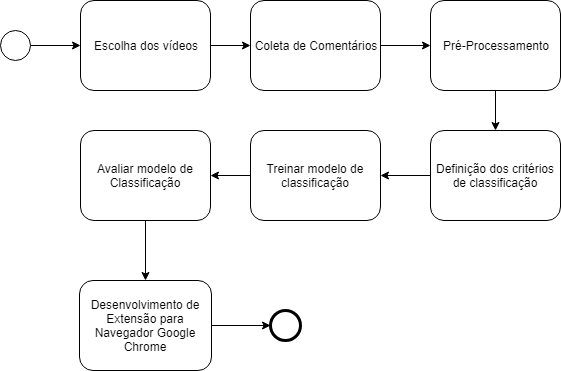
\includegraphics[scale=0.7]{figuras/figura_6.png} % altere o atributo scale para o tamanho da figura
	\end{center}
	\legend{Fonte: autor}
%Verificar se precisa por a data aqui 
\end{figure}


% Passos sugeridos de acordo com os objetivos específicos:
% Classificar os comentários: (1) Coleta de Dados (2) Pré-Processamento (3) Definição dos Critérios de Classificação
% Analisar os comentários: (4) Treinamento do Modelo de Classificação
% Indicar os vídeos Pejorativos (5) xxxxxx
% Avaliar o modelo de classificação (6) Avaliação do Modelo de Classificação
\subsection{Escolha dos vídeos}
O principal critério para a escolha do vídeo para este trabalho, é que seu público alvo seja infantil ou adolescente. Naturalmente, quanto mais comentários o vídeo possuir, maior a quantidade de dados para análise, logo o ideal foi buscar vídeos infantis que apresentavam um número expressivo de comentários, em torno de pelo menos mil. Porém nem sempre foi possível encontrar vídeos com essa quantidade ideal de comentários, o que não impediu que também fossem utilizados. A popularidade do canal que postou o vídeo foi um fator  considerado, visto que um canal com maior popularidade também  possui vídeos com mais comentários.


\subsection{Coleta de Dados}
A fim de ter os dados para o ponto de partida da pesquisa e tendo em conta a grande quantidade de comentários em vídeos com público-alvo jovem, foi desenvolvida uma ferramenta em Python para coleta dos comentários em vídeos do Youtube. O objetivo da ferramenta é ser simples e objetiva na coleta desses comentários.

A aplicação desenvolvida pelo autor, utiliza a API do Youtube (Versão 3) e permite tanto obter os comentários de topo (\textit{top level comments} ou \textit{Comment Threads}), como as réplicas à esses comentários, dado o ID do vídeo que pode ser encontrado na sua URL, permitindo obter todos os comentários públicos disponíveis no vídeo, até o momento da coleta. O código fonte para a aplicação pode ser encontrado em: \footnote{https://github.com/ssisaias/ytCommentMiner}.


\subsection{Pré-Processamento}
Uma vez que os dados armazenados não estão em formato adequado para extração do conhecimento, faz-se necessária a aplicação de métodos para \textit{extração, integração,} \textit{transformação},
% ta mas o que é isso? ai vou preicsar olhar no referencial teórico e adaptar conforme o que eu fiz aqui!!!
\textit{limpeza}, \textit{seleção e redução} de volume desses dados, antes da etapa de mineração \cite{morais2007mineraccao}.

Inicialmente, observa-se uma grande quantidade de comentários sem sentido em vídeos infantis no Youtube, compostos quase que inteiramente por espaços em branco ou símbolos e letras aleatórios. Em vídeos destinados à adolescentes, há menor ocorrência de comentários sem sentido. 

Nesta etapa, um \textit{script} escrito em Python foi executado para extrair somente os textos dos comentários obtidos através da ferramenta de extração. Em seguida, através da ferramenta NLTK, o pré-processamento foi realizado: os acentos foram removidos e os textos foram \textit{tokenizados}, através de um processo que remove palavras sem valor semântico para o classificador e reduz palavras com valor semântico ao seu radical.

Vale notar que a API do Youtube também retorna o texto dos comentários contendo caracteres unicode, que representam letras acentuadas e alguns poucos símbolos, como apóstrofo (') e \textit{ampersand} (\&). Ao utilizar a versão 3 da linguagem Python, os caracteres unicode são automaticamente substituídos pelo caractere correspondente na língua portuguesa, podendo assim os textos, seguirem adiante na etapas de processamento.


\subsection{Definição dos Critérios de Classificação}

A classificação dos comentários é definida manualmente, levando em consideração comentários de amostragem, que foram classificados como \textbf{pejorativos} ou \textbf{não pejorativos}. 

Dado a enorme quantidade de comentários coletados, um dicionário de classificação também foi criado para a ferramenta \textbf{SentiStrength}, a fim de facilitar a criação do conjunto de treino a ser dado de entrada para gerar o modelo de classificação. % O dicionário pode ser verificado no apendice X. (colocar a referencia ao apendice aqui)

Após a classificação manual e a classificação assistida utilizando a SentiStrength, um modelo foi treinado para que possa classificar automaticamente os novos comentários obtidos do Youtube.

\subsection{Treinamento do Modelo de Classificação}
O classificador Naïve Bayes recebe um conjunto de dados de treino, e um conjunto de testes para averiguar a precisão do modelo de classificação \cite{ZhangandLi2007Bayes}. Esses conjuntos de dados foram escolhidos de forma aleatória dentre os comentários obtidos para o vídeo \textbf{Não Faz Sentido! - Crepúsculo [+13]}, sendo utilizados aproximadamente 50\% (32.131) para grupo de treino e 50\% (32.130) para grupo de testes. 

Utilizando a SentiStrength obteve-se inicialmente uma classificação automática do grupo de treino. Essa classificação foi averiguada pelo autor e melhorada, afim de tornar o modelo mais preciso. Por exemplo, comentários identificados erroneamente como pejorativos foram trocados manualmente para neutros e vice-versa.

\subsection{Avaliação do Modelo de Classificação}
%O conhecimento extraído na fase de mineração de dados pode gerar uma grande quantidade de padrões \cite{morais2007mineraccao}.

O modelo gerado é enfim testado utilizando os comentários que não foram utilizados na fase de treino, ou seja, utilizando os comentários selecionados para compor o conjunto de teste. 

O modelo também foi utilizado nos outros grupos de comentários obtidos, afim de obter a classificação para os outros vídeos analisados. Vale notar que para estes conjunto de comentários a única etapa não realizada dentre os procedimentos mencionados neste Capítulo foi a geração do modelo, ou seja, estes comentários foram pré-processados, classificados pela ferramente SentiStrength, analisados pelo autor, classificados pelo modelo de classificação e por fim tiveram os resultados obtidos comparados com o esperado.

A avaliação do modelo é feita através da ferramenta Scikit Learn, que fornece métodos de \textit{score} prontos para as medidas de \textit{precision} e \textit{recall}. Os resultados da avaliação são apresentados no Capítulo 6.

%preciso mencionar elas lá em cima, quando for falar do scikit. % talvez colocar alguma referencia aqui seja bom tb

%O modelo de classificação gerado agora pode ser testado utilizando todos os comentários que foram coletados afim de chegar as conclusões sobre os tipos de comentários realizados em vídeos infantis e o grau de segurança da seção de comentários de cada vídeo.
\begin{comment}
\subsection{Indicar vídeos com comentários pejorativos}
Nessa etapa, iremos avaliar os resultados do processamento dos comentários, agregando agora pelos vídeos dos quais foram coletados, indicando quais os vídeos tem maiores taxas de comentários pejorativos e que não são considerados seguros para crianças e adolescentes.
\end{comment}


\subsection{Criação de extensão para Google Chrome}

Ao obter o modelo de classificação, foi desenvolvida uma extensão do navegador da web Google Chrome que se utiliza de um \textit{Web Service} que retorna a margem de comentários negativos e positivos para o vídeo sendo assistido naquele momento. 

Caso os comentários do vídeo ainda não tenham sido classificados, o serviço irá iniciar um procedimento automático de classificação, tornando os resultados disponíveis dentro de no máximo algumas horas.

A Figura \ref{fig:chrome_plugin} mostra um exemplo de classificação retornada pela extensão em um vídeo do Youtube.

\begin{figure}[H] %use h para forçar que a figura fique abaixo do texto
	\caption{\label{fig:chrome_plugin} Extensão do Google Chrome}
	\begin{center}
	    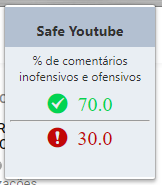
\includegraphics[scale=1.2]{figuras/extensao_chrome.PNG} % altere o atributo scale para o tamanho da figura
	\end{center}
	\legend{Fonte: Autor}
%Verificar se precisa por a data aqui 
\end{figure}

Os códigos da extensão \footnote{https://github.com/ssisaias/safe-youtube} e do serviço web \footnote{https://github.com/ssisaias/safe-youtube-service}, estão disponíveis publicamente e podem ser encontrados na plataforma Github.
\textcolor{green}{posso falar que não é o foco da pesquisa a avaliação da extensão, e que é tipo algo como um bônus, um produto?}

\begin{comment}
\textit{A última Seção dos procedimentos é o cronograma. Apresente a versão que entregará à banca ao final do semestre. Se seus procedimentos não estiverem organizados em subseções, esta será a subseção 4.1. Após ler, remova este texto explicativo.}
\end{comment}

% TCC 2 - remove cronograma
\begin{comment}
\subsection{Cronograma}

\begin{table}[H]
\centering
\resizebox{\textwidth}{!}{\begin{tabular}{|l|c|c|c|c|c|c|c|c|c|c|c|c|c|c|c|c|c|c|c|c|c|}
\hline
\multicolumn{1}{|c|}{\multirow{2}{*}{ATIVIDADES}} & \multicolumn{8}{|c|}{2017}  & \multicolumn{12}{c|}{2018}  \\ \cline{2-21} 
\multicolumn{1}{|c|}{} & 
\multicolumn{2}{c|}{Set} &
\multicolumn{2}{c|}{Out} & 
\multicolumn{2}{c|}{Nov} & 
\multicolumn{2}{c|}{Dez} & 
\multicolumn{2}{c|}{Fev} & 
\multicolumn{2}{c|}{Mar} &
\multicolumn{2}{c|}{Abr} & 
\multicolumn{2}{c|}{Mai} &
\multicolumn{2}{c|}{Jun} &
\multicolumn{2}{c|}{Jul}\\ \hline
\begin{tabular}[c]{@{}l@{}}Definição do projeto\end{tabular} & x &  &  &  &  &  &  & - & & &  &  &  &  &  &  & &  &  &\\ \hline
Coleta inicial dos comentários &  & x &  &  &  &  &  & - &  &  &  &  &  & & & & &  & &\\ \hline
Pesquisa e definição do referencial teórico &  &  & x & x &  &  &  & - &  &  &  &  &  & & & & &  &  &\\ \hline
Escrita do TCC I &  & x & x & x & x & x &  & - &  &  &  &  &  & & & & &   &  &\\ \hline
Defesa do TCC I &  &  &  &  &  &  & x & - &  &  &  &  &  & & & & &  &  &\\ \hline
Escolha dos vídeos &  &  &  &  &  &  &  & - & x &  &  &  &  & & & & &   &  &\\ \hline
Coleta de comentários do Youtube &  &  &  &  &  &  &  & - &  & x &  &  &  & & & & &   &  &\\ \hline
Pré Processamento dos comentários &  &  &  &  &  &  &  & - &  &  & x & x &  &  & & & &  &  &\\ \hline
Treino do modelo de classificação &  &  &  &  &  &  &  & - &  &  &  &  & x & x &  &  & &   &  &\\ \hline
Avaliação do modelo de classificação &  &  &  &  &  &  &  & - &  &  &  &  &  &  & x & x & x &  &  & \\ \hline
Indicar vídeos com comentários pejorativos &  &  &  &  &  &  &  & - &  &  &  &  &  &  & &  &  & x &  &\\ \hline
Defesa da Monografia &  &  &  &  &  &  &  & - &  &  &  &  &  &  & & &  &  & x &\\ \hline
\end{tabular}}
\end{table}

\end{comment}
